% This is samplepaper.tex, a sample chapter demonstrating the
% LLNCS macro package for Springer Computer Science proceedings;
% Version 2.20 of 2017/10/04
%
\documentclass[runningheads]{llncs}
%

\usepackage{cite}
\usepackage{caption}


\usepackage{amsmath,amssymb}
\usepackage{siunitx}
\usepackage{subfig}
\usepackage{graphicx}
% Used for displaying a sample figure. If possible, figure files should
% be included in EPS format.
%
% If you use the hyperref package, please uncomment the following line
% to display URLs in blue roman font according to Springer's eBook style:
% \renewcommand\UrlFont{\color{blue}\rmfamily}

\begin{document}
%
\title{Acoustic SLAM for Unprepared Environments with Gaussian Processes}
%
%\titlerunning{Abbreviated paper title}
% If the paper title is too long for the running head, you can set
% an abbreviated paper title here
%
\author{B. Sc. Oliver Neumann \\
Dipl. Phys. Jana Mayer \\
Dr. Ing. Benjamin Noack}

\institute{
	Karlsruhe Institute of Technologie (KIT) \\
	Institute for Anthropomatics and Robotics (IAR) \\
	Intelligent Sensor-Actuator-Systems (ISAS) \\
	Adenauerring 2 76131 Karlsruhe Germany}
%
\maketitle              % typeset the header of the contribution
%

\begin{abstract}

% SLAM
Simultaneous localization and mapping (SLAM) became one of the most important research fields in robotics. Modern approaches of SLAM are based on discrete landmarks that are used to estimate the position of the actor. But there are environments where no landmarks could be detected or the landmarks are not suitable for accurate localization.
% From discrete to continuous
Instead of discrete landmarks, researchers used physical phenomena as continuous functions for localization purposes. The continuous function is usually approximated with a Gaussian process as the map. Measurements then will be fused with an estimated position (e.g. from an inertial measurement unit) to increase accuracy.
% Vision
Those approaches have promising performance and there are a lot of use cases. From indoor robot cleaning to autonomous submarines for undersea pipeline investigation up to autonomous drones for weather observation.
% Aim
In this project we want to investigate if a speaker and microphone together with an inertial measurement unit (IMU)  mounted on a robot, is capable of localizing itself in an unprepared environment. Therefore a specific signal will be sent via the speaker and from the microphone input, a continuous function will be derived based on the concept of room impulse response.  This function will be approximated with Gaussian processes and should be used as input for SLAM.

\end{abstract}

\section{Motivation}

% SLAM
Robots often have to act in an unknown environment. For that, a robot has to recognize the environment and locate itself in it. For example, an actor wants to find the dishwasher to clean up the kitchen. This problem is also known as simultaneous localization and mapping (SLAM) in the context of robotics. Common approaches using discrete landmarks recognized by the robot to set up a landmark map of the environment (see Figure \ref{fig:grisetti_slam_example}). With this map of landmarks, it's possible to estimate the position of the robot. A typical example of landmarks are features from images, which are taken by a camera from the robot.

% From discrete to continuous
For SLAM there are a variety of use cases but there are also scenarios where it's not possible to obtain landmarks that are suitable for SLAM approaches. For example, at the sea, water is usually muddy and cameras would only see over a short distance. There it wouldn't be possible to extract image features suitable for SLAM approaches. That's where scientists switched from discrete landmarks to continuous functions given by physical phenomena. A common approach is to use the magnetic field for indoor localization \cite{kok_scalable_2018}. This is also a good example to show also what performance such approaches could have.

% Vision
But it's not only a workaround to use SLAM in situations, where discrete landmarks are not possible to obtain. Continuous approaches could be as good as discrete ones and in combination, they could be even better. Also, when it comes to costs if the aim of a robot is to measure physical phenomena, why don't use this data for SLAM instead of buying a camera and more expensive hardware for real-time feature extraction of the images.

% Science question
There is a huge potential of SLAM with continuous functions and the science community is only at the beginning. This project wants to examine if an actor could locate itself in an unprepared unknown environment only by using a microphone, speaker and inertial measurement unit (IMU). For that, the speaker sends out a signal which is received by the microphone. But the signal will be changed mainly because of interference of the signal with the room. 

% Aims and Tasks
One Task is now to derive a continuous function from the microphone signal. For that, the room will be treated as an electrical system. The signal from the speaker will be the input and the microphone signal the output of the system. So an impulse response could be calculated. This concept is known as the room impulse response (RIR) \cite{dokmanic_roomrecslam_2016}. Based on that, various continuous functions have to be validated which one is the best for indoor SLAM approaches. For example, using only the ten highest peaks of the RIR. But before that, data has to be recorded for analysis, test and validation purposes. At the end of this project, the performance of this indoor SLAM approach should be compared to others. Therefore approaches described in Chapter \ref{chap:stat_of_the_art} should be used.

\begin{figure}[h!]
	\centering
	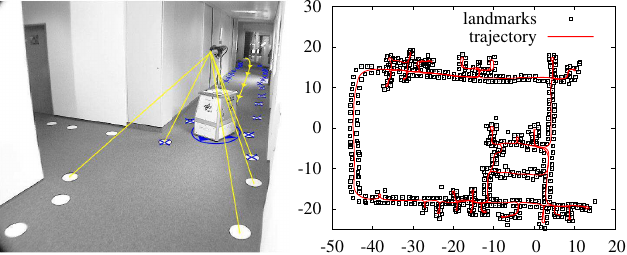
\includegraphics[width=0.935\textwidth]{images/grisetti_slam_example.png}
	\caption{
		An illustration for SLAM with a prepared environment for the robot. Landmarks are mounted on the floor which the robot can recognize (left image). The generated map is shown on the right \cite{grisetti_tutorial_2010}.
	}
	\label{fig:grisetti_slam_example}
\end{figure}
\section{Preliminaries}

SLAM describes the field of problems where an agent has to locate itself in an unknown environment. Therefore a map of the environment has to be created where the actor can locate itself \cite{grisetti_tutorial_2010}. The map could consist of discrete landmarks, continuous functions, but also planes as an approximation of the environment. There are several SLAM approaches. Usually all measurements, as well as agent positions, are Gaussian distributed. That's why the map is only an estimation and all SLAM approaches itself are probabilistic approaches \cite{grisetti_tutorial_2010}.

SLAM could be subdivided into two common classes \cite{grisetti_tutorial_2010}. First, approaches where only the most probable current position of the agent within the map is wanted, are called filtering or on-line SLAM approaches. In contrast to that, when the current most probable full trajectory of the robot within the map is calculated, those approaches are called smoothing or full SLAM. Both approaches acting in real-time but only smoothing approaches calculating a full trajectory of the robot which could change over time.

Regardless of filtering or smoothing approaches, they often use Kalman or particle filter for current state estimation \cite{grisetti_tutorial_2010}. Kalman filter is a mathematical concept consists of two steps \cite{kalman1960}. The prediction and update steps. In the prediction, the next state is predicted by using all data given until this timestep. In the update phase, the predicted state is improved by combining it with the new measured state. By changing the parameters it can be controlled if the Kalman filter should trust more the predictions or measurements. It is suggestive to trust more the predictions if the measurements are normally distributed with a large covariance. If the measurements have nearly no uncertainty, it would be better to trust the measurements. Kalman filter is a famous concept in the science community. 

\begin{figure}[h!]
	\centering
	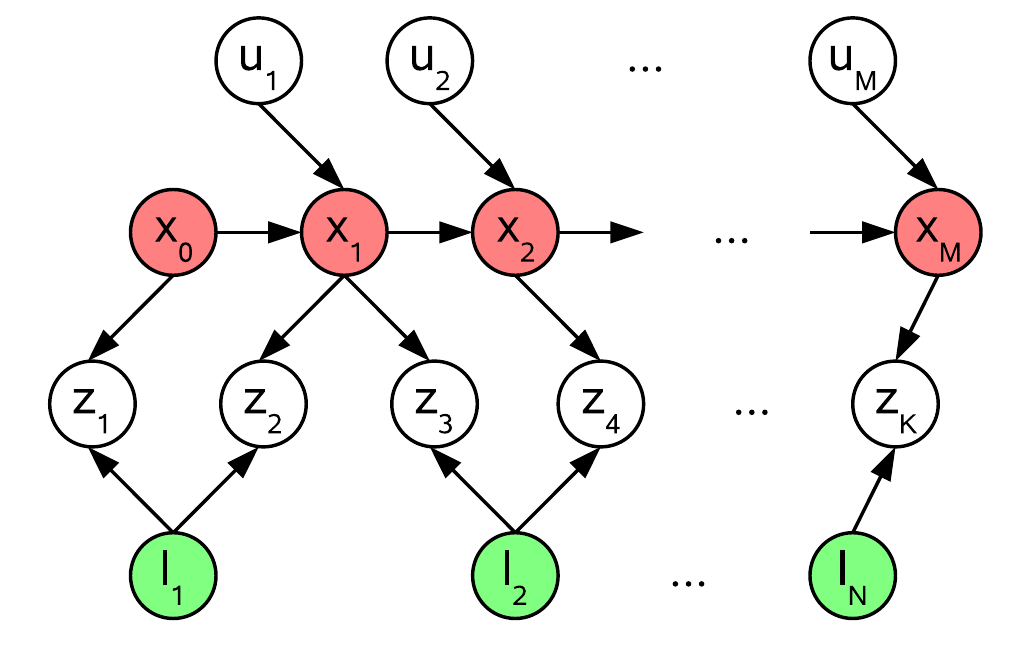
\includegraphics[width=0.4\textwidth]{images/kaess_slam_graph.png}
	\caption{
		SLAM graph with $x_i$ as the robot position at time step $i$. $l_j$ is the $j^{th}$ landmark. $z_k$ is the $k^{th}$ by the robot measured landmark. $u_i$ is the control input at time step $i$ which is for example odometry data \cite{kaess_isam:_2008}. For understanding: At time step $1$ the robot position was $x_1$ and it measured landmark $l_1$ and $l_2$ which can be seen by the measurements $z_2$ and $z_3$. The input from the control unit was $u_1$.
	}
	\label{fig:kaess_slam_graph}
\end{figure}

One large disadvantage is that Kalman filters are only following one hypothesis. For example, when tracking a car at a crossing it could be better to follow the hypothesis, that the car is going straight, but also the hypothesis that the car will turn right or left. When tracking using the Kalman filter, the car could be lost after the crossing. That's where the concept of particle filters was introduced \cite{qun_particle_filter}. In contrast to Kalman filters, particle filters can follow multiple hypotheses. To be exact, each particle can follow one hypothesis.

State-of-the-art SLAM techniques using graph-based approaches. While the robot is moving and making measurements a graph is build up as illustrated in figure \ref{fig:kaess_slam_graph}. With modern graph algorithms the position $x_0, ... , x_n$ can now be estimated. In figure \ref{fig:grisetti_slam_showcase} the performance of those approaches is illustrated.

\begin{figure}[h!]
	\centering
	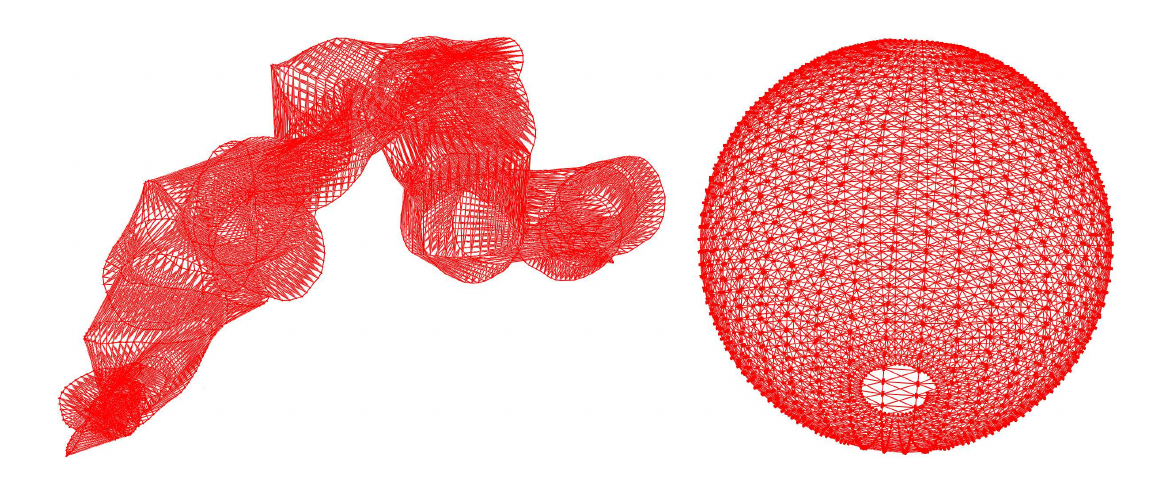
\includegraphics[width=\textwidth]{images/grisetti_slam_showcase.png}
	\caption{
		A showcase of a current state-of-the-art graph-based SLAM approach. Initial position estimation on the left and next to it graph-based SLAM position estimation. The robot was moved in a simulation on the surface of a sphere \cite{grisetti_tutorial_2010}.
	}
	\label{fig:grisetti_slam_showcase}
\end{figure}

When switching from discrete landmarks to continuous functions, these functions need to be approximated within the area of the environment. So it is possible to have values between the measurements which is necessary to improve the position estimation of the actor. When knowing the input space (in this case the environment) but don't want to make any assumptions to the underlying function, Gaussian processes (GP) are the solution \cite{ebden_gaussian_2015}.

Basically, GP are defined by a mean function $m(x) = \mathbb{E}(y(x))$ and a covariance function $k(x_i, x_j) = \mathbb{E}((y(x_i) - m(x_i)) (y(x_j) - m(x_j)))$ also called the kernel. If $m(x) = 0$ the GP are called centered. For the kernel, radial basis functions can be used which means $k(x_i, x_j) = k(||x_i - x_j||)$. Such GP are called radial. One very common radial kernel is the squared exponential kernel \cite{ebden_gaussian_2015}

$$
k(x_i, x_j) = \sigma ^2 \exp 
\begin{pmatrix}
-\frac{(x_i - x_j)^2}{2l^2}
\end{pmatrix}\text{.}
$$

As mentioned before, for SLAM it should be possible to model normally distributed measurements. GP can model normally distributed uncertainty. Assume the noise is normally distributed with variance $\sigma^2_{noise}$. Then measurements can be described as $y_i = f(x_i) + \mathcal{N}(0, \sigma^2_{noise})$. Combining the covariance function with the model of noisy measurements, that will lead to the slightly changed kernel
$$
k(x_i, x_j) = \sigma ^2 \exp 
\begin{pmatrix}
-\frac{(x_i - x_j)^2}{2l^2}
\end{pmatrix}
+ \delta_{ij} \sigma^2_{noise}
$$
where $\delta_{ij}$ is the Kronecker delta. This function is only $1$ when $i=j$ otherwise it is $0$. So, the covariance $k(x_i, x_j)$ is only increased by $\sigma^2_{noise}$ when $i=j$. That means the uncertainty increases for $k(x_i, x_i)$ which are the measurements. Figure \ref{fig:gaussian_process_example} gives an example of GP with and without noisy measurements.

Assume now there are $n$ measurements $y_1, ..., y_n$ taken at $x_1, ..., x_n$. Then the covariance matrix would be
$$
K = \begin{bmatrix}
k(x_1, x_1) & k(x_1, x_2) & \dots & k(x_1, x_n) \\
k(x_2, x_1) & k(x_2, x_2) & \dots & k(x_2, x_n) \\
\vdots & \vdots & \ddots & \vdots \\
k(x_n, x_1) & k(x_n, x_2) & \dots & k(x_n, x_n) \\
\end{bmatrix}\text{.}
$$
Because of GP modeling data from a multivariate normal distribution, $y$ and $y_*$ can be modeled as
$$
\begin{bmatrix}
y \\
y_* \\
\end{bmatrix} 
\sim
\mathcal{N} 
\begin{pmatrix}
0, 
\begin{bmatrix}
K & K_*^T \\
K_* & K_{**} \\
\end{bmatrix}
\end{pmatrix}\text{with}
$$
$$
K_* = [k(x_*, x_1), \dots, k(x_*, x_n)],
$$
$$
K_{**} = k(x_*, x_*)\text{.}
$$
Using the mathematics of multivariate Gaussian distributions, the most likely value of $y_*$ can be calculated by
$$
y_*|y \sim \mathcal{N}(K_*K^{-1}y, K_{**} - K_*K^{-1}K_*^T)
$$
$$
\Rightarrow {y}_* = m(x_*) = K_*K^{-1}y\text{ .}
$$
The derivation of the formula is well explained by Ebden \cite{ebden_gaussian_2015}. Notice that also the variance for $y_*$ is given by
$$
var(y_*) = K_{**} - K_*K^{-1}K_*^T\text{ .}
$$

\begin{figure}[h!]
	\centering	
	\subfloat{{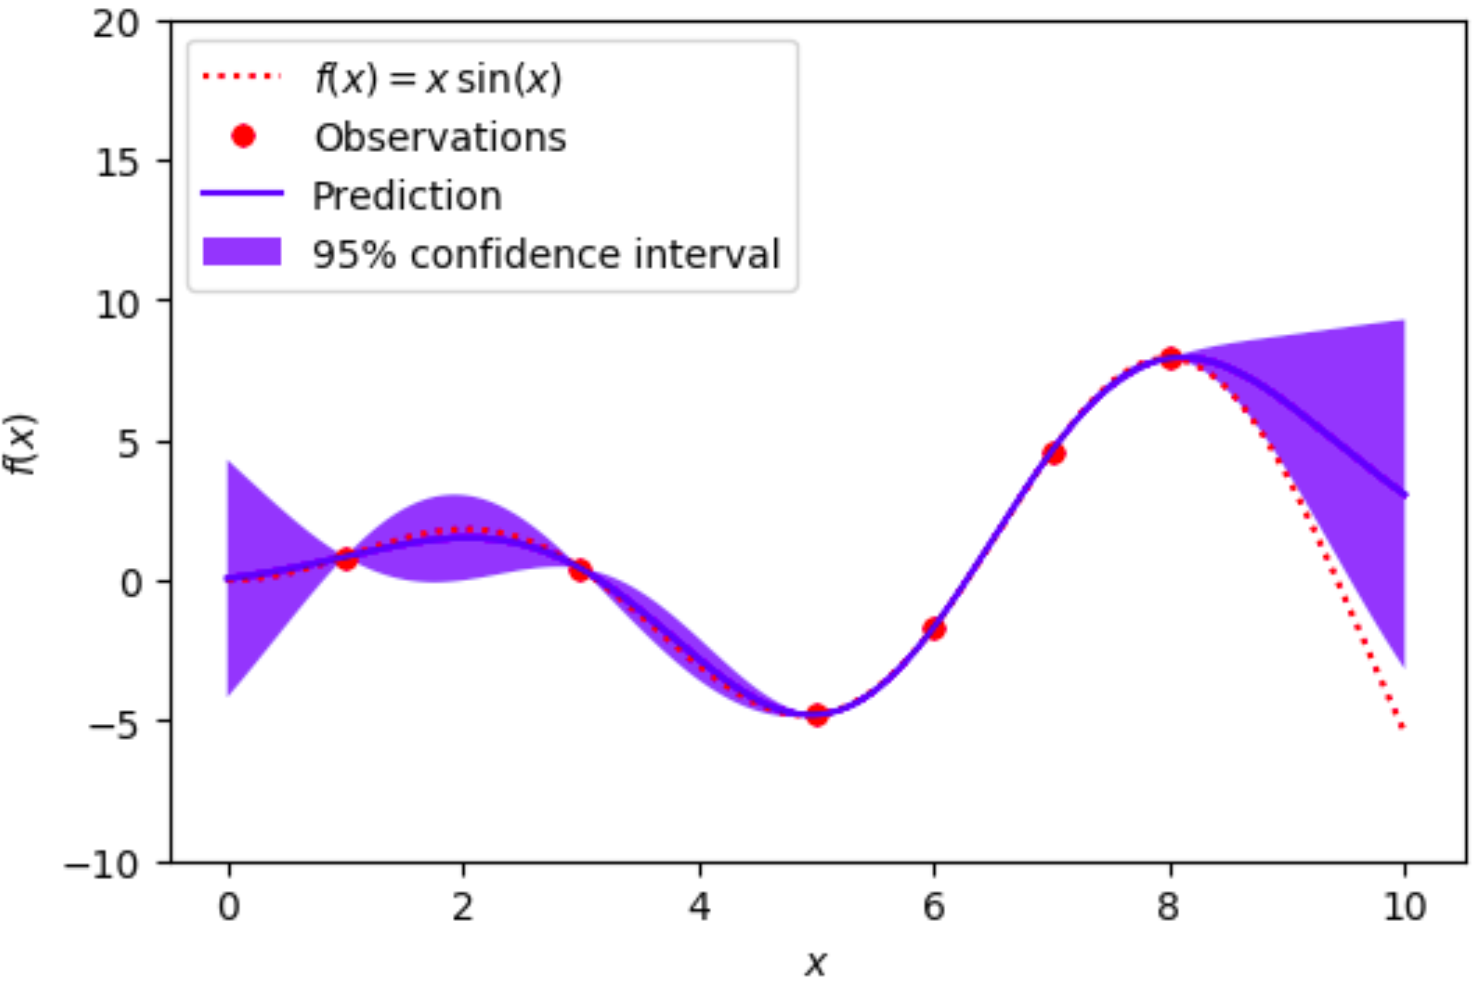
\includegraphics[width=0.5\textwidth]{images/gaussian_process_example1.png} }}
	\subfloat{{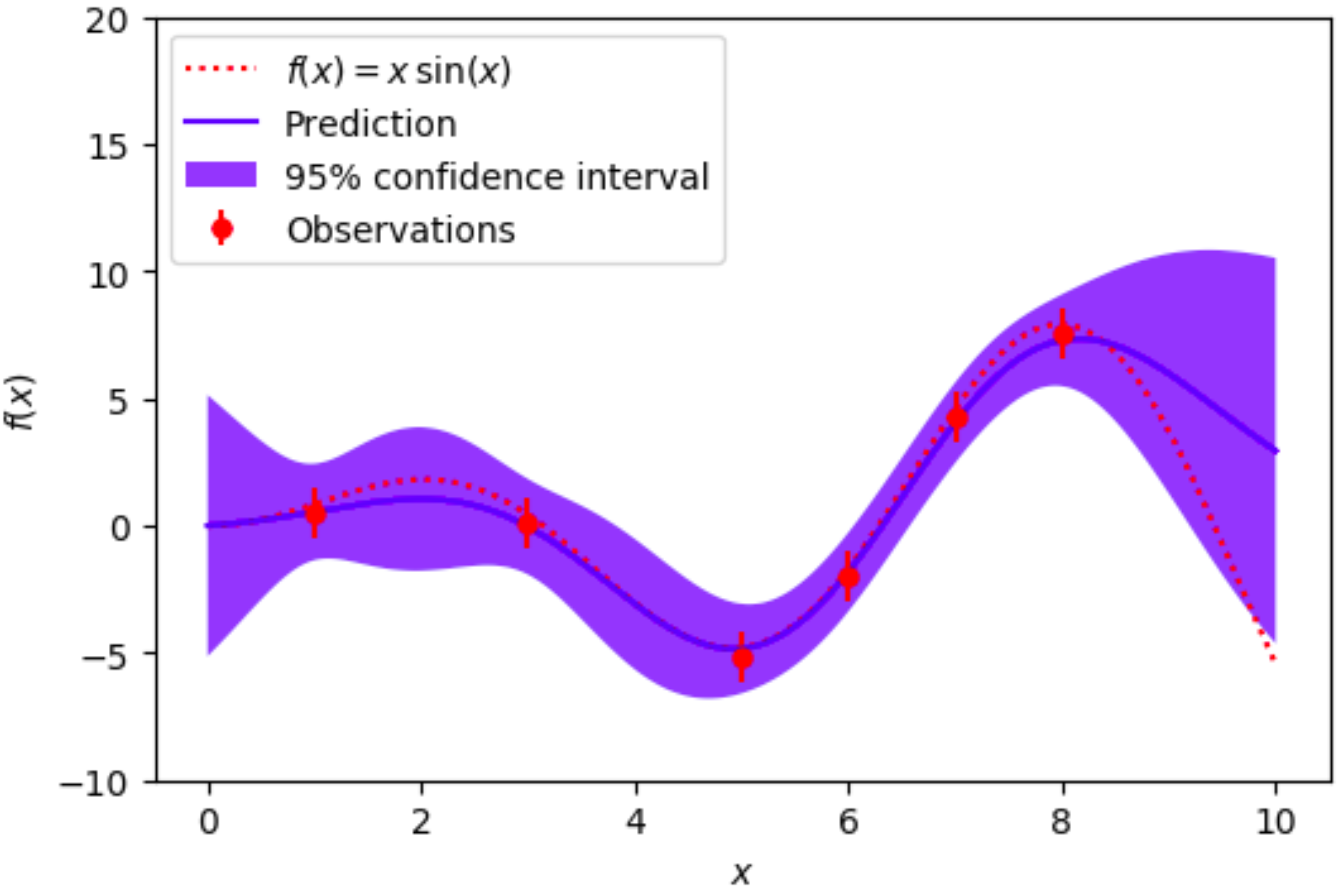
\includegraphics[width=0.5\textwidth]{images/gaussian_process_example2.png} }}
	\caption{
		A plot of two GP regressions with the same measurements $f(x_i)$ but the one at the right has noisy measurements with variance $\sigma_{noise}^2 = 1$. The uncertainty is represented through the confidence interval.
	}
	\label{fig:gaussian_process_example}
\end{figure}

An example of uncertainty in measurements, prediction of $y_*$ and probability of the prediction can be seen in Figure \ref{fig:gaussian_process_example}. Note that for linear increasing number of measurements the size of the covariance matrix rises quadratically and for $y_*$ the inverse of that matrix has to be calculated. So it is computational expensive for large-scale data. There are approaches which facing that problem. Another remark is that the standard GP is not possible to model uncertainty in the input data. So it is not possible to model uncertainty in the position of the robot with GP. 

\section{State of the Art}
\label{chap:stat_of_the_art}

In this Chapter, some recent SLAM approaches based on continuous functions will be presented. It exemplifies what performance current approaches have and on what work this project is based on. 

\subsection{Scalable Magnetic Field SLAM}
\label{sec:scalable_magnetic_slam}

One impressing approach from Kok et al. showing full SLAM in 3D using the magnetic field and GP \cite{kok_scalable_2018}. The magnetic field was approximated with GP and because of performance issues the environment is divided in 3D hexagons as illustrated in figure \ref{fig:kok_example}. So there is a GP for each hexagonal region. This reduces the size of the covariance matrix for each GP and increases performance. 

To approximate the magnetic field, they use a combination of two kernels, the linear and squared exponential kernel and a mean centered around zero \cite{kok_scalable_2018}, that leads to the 
following Gaussian process
$$
GP(0, k_{lin}(x_i, x_j) + k_{se}(x_i, x_j)) \text{ with}
$$
$$
k_{lin}(x_i, x_j) = \sigma_{lin}^2 x_i^T x_j, 
$$
$$
k_{se} = \sigma_{se}^2 \exp 
\begin{pmatrix}
-\frac{||x_i - x_j||^2}{2l^2}
\end{pmatrix}\text{.}
$$

For position estimation, Kok et al. don't use any graph-based approach. Instead, they use a combination of Kalman and particle filter. To update measurements a Kalman filter is used. For predictions in time particle filters are used. A detailed description can be found in their paper \cite{kok_scalable_2018}. Figure \ref{fig:kok_example} demonstrates the performance of their approach. This paper shows vivid what SLAM approaches with continuous functions are capable of.

\begin{figure}[h!]
	\centering
	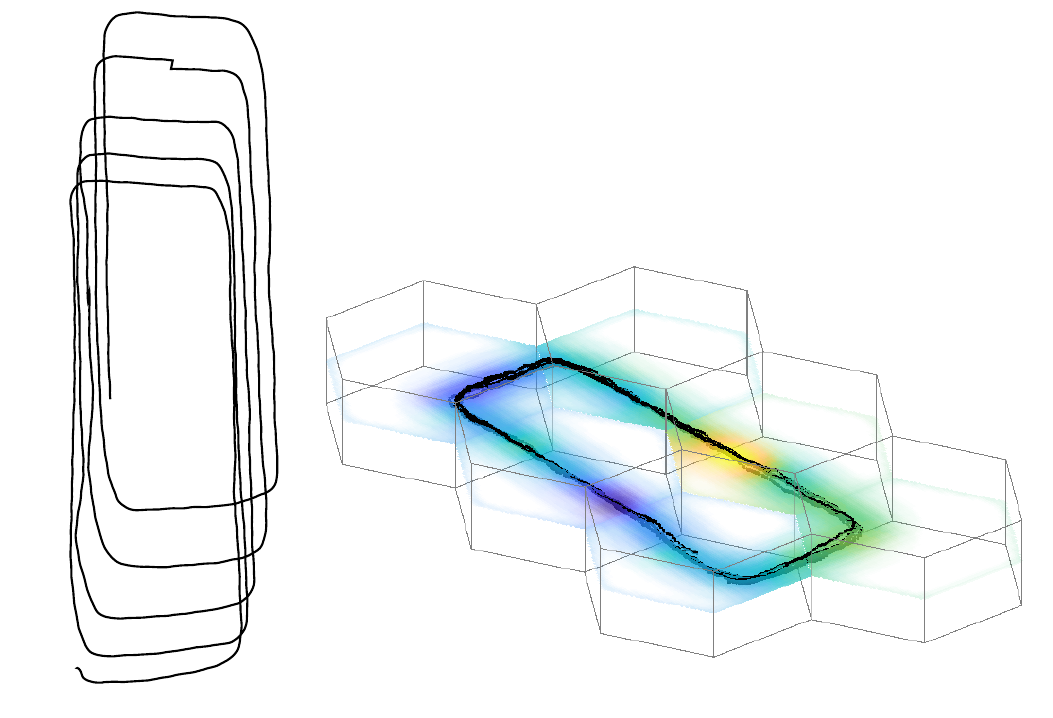
\includegraphics[width=0.8\textwidth]{images/kok_example.png}
	\caption{
		Performance demonstration of the SLAM algorithm by Kok et al. \cite{kok_scalable_2018}. The trajectory on the left shows the odometry data collected by an iPhone 6s and next to it the resulting trajectory with the approximated magnetic field.
	}
	\label{fig:kok_example}
\end{figure}

\newpage
\subsection{Terrain Field SLAM}
\label{sec:terrain_slam}
Another interesting approach from Yu et al. shows which different continuous functions could be used for SLAM \cite{yu_terrain_2018}. In their paper, they described a SLAM algorithm where the continuous function is the vibration caused by the interaction between the robot and the terrain. Their experimental setup and the robot can be seen in figure \ref{fig:yu_setup}.

\begin{figure}[h!]
	\centering
	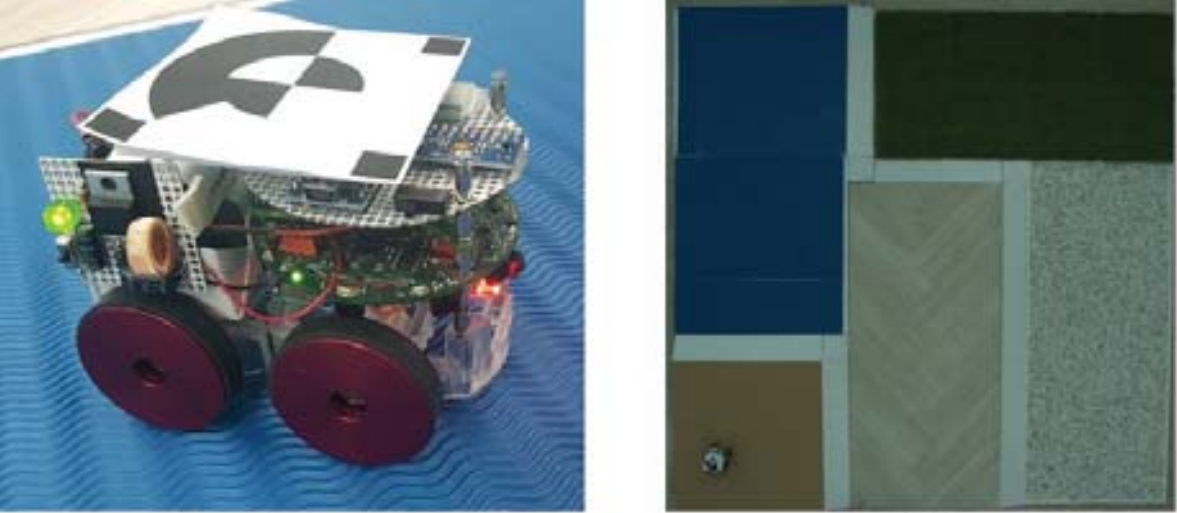
\includegraphics[width=0.8\textwidth]{images/yu_setup.png}
	\caption{
		Illustration of the setup by Yu et al. \cite{yu_terrain_2018}. The mobile robot at the left and
		on the right the environment for the robot to move in. The environment containing
		five different subsurfaces.
	}
	\label{fig:yu_setup}
\end{figure}

Yu et al. also used GP to infer the terrain field. A performance demonstration can be seen in figure \ref{fig:yu_performance}. Even if they don't face the problem of doing SLAM and Gaussian regression on-line and there is a little deviation over time, the results are considerable.


\begin{figure}[h!]
	\centering
	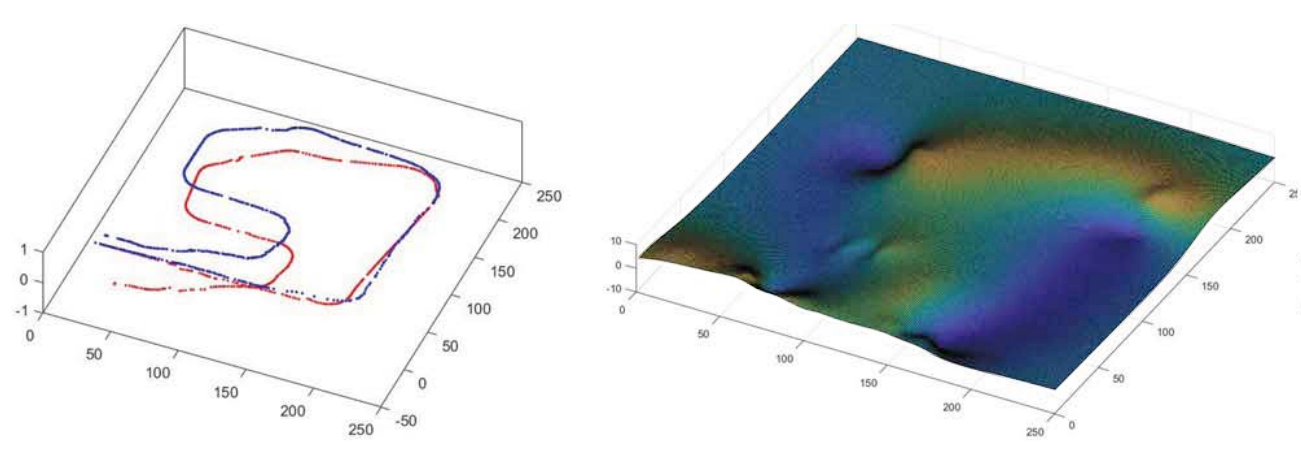
\includegraphics[width=\textwidth]{images/yu_performance.png}
	\caption{
		Performance illustration of the terrain based SLAM approach by Yu et al. \cite{yu_terrain_2018}.
		Robot trajectory (red) on the left and ground truth (blue). Righ shows inferred terrain field.
	}
	\label{fig:yu_performance}
\end{figure}

\subsection{Acoustic SLAM}
\label{sec:acoustic_slam}

When thinking about other potential phenomena for SLAM approaches, acoustic would be a good option. Speakers are cheap and normally a lot of electronic devices have one. Also, acoustic approaches could be used underwater in contrast to camera-based SLAM or the approaches described in Section \ref{sec:scalable_magnetic_slam} and \ref{sec:terrain_slam}.

What nearly all acoustic-based approaches have in common, that they have a prepared environment. Evers et al. in their paper about A-SLAM \cite{evers_aslam_2016} is a good example. They use speakers placed in a room emitting a specific signal and an actor equipped with a microphone array to calculate the incoming directions of the speaker signals. Each speaker acts as a landmark which position has to be estimated so it shouldn't move over time. Although it is a landmark-based approach, it shows what performance an acoustic-based SLAM could have.

\begin{figure}[h!]
	\centering
	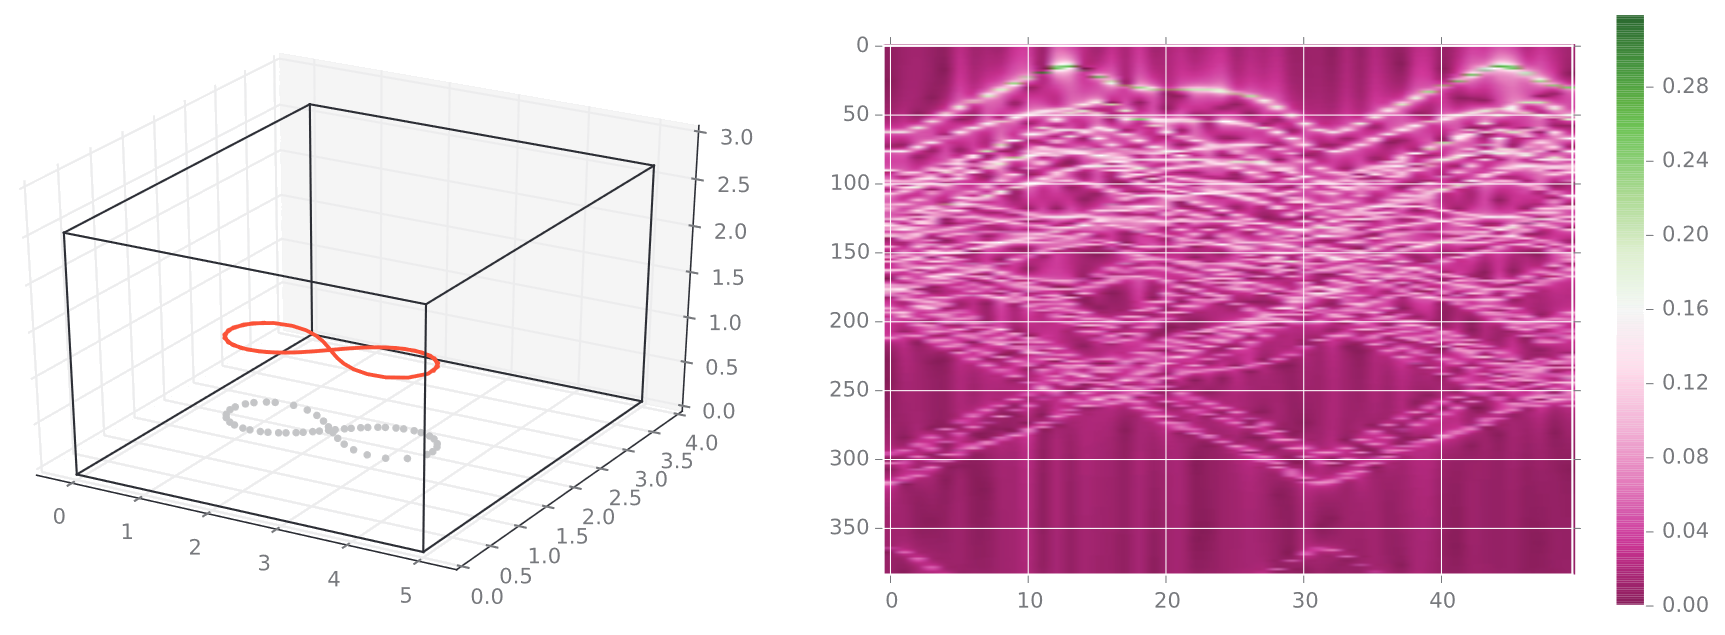
\includegraphics[width=\textwidth]{images/acoustic_slam.png}
	\caption{
		RIR illustration of Dokmanic et al. \cite{dokmanic_roomrecslam_2016}. Left Image shows the trajectory in red of the robot. At the right a plot of the RIR where x-axis is the time and y-axis the RIR.
	}
	\label{fig:dokmanic_roomrecslam}
\end{figure}

There are also acoustic SLAM approaches based on continuous functions. One is from Dokmanic et al. who use the concept of room impulse response (RIR) from room reconstruction for a SLAM approach \cite{dokmanic_roomrecslam_2016}. Therefore he placed a speaker in the room which is sending a specific signal. An actor can now move around and calculate the RIR based on the current position. This RIR is used for SLAM. One thing to point out that in this paper the RIR is a smooth continuous function when the robot is moving and when the robot passes the same point the RIR will be similar (see Figure \ref{fig:dokmanic_roomrecslam}).

\section{Pre-Studies}
\label{chap:pre_studies}

Based on the work of Dokmanic et al. \cite{dokmanic_roomrecslam_2016} the question is now if the RIR will also be suitable for SLAM when the speaker is also mounted on the robot. In the case of Dokmanic et al. \cite{dokmanic_roomrecslam_2016} described in section \ref{sec:acoustic_slam}, the RIR is a continuous function that won't change until the speaker moves or the room will change. In this project, the speaker will move along with the robot. So the RIR as a 2D function over the room will change every time. In the pre-studies, it will be investigated if the RIR is suitable for SLAM when measuring the RIR at the position of a moving speaker.

But first a short recap of the room impulse response (RIR). The principle of sending a signal in a room and recording it with a microphone could be treated as an electrical system where the sent signal is the input and the recorded signal the output of the electrical system. In the concept of electrical systems, the output $y(t)$ depends on the input $x(t)$ and a function $g(t)$ which is convolved with the input in time space. So it follows
$$
y(t) = (g * x)(t) \text{.}
$$

When now stimulating the system with an infinite small function also called impulse, the function $g(t)$ is called the impulse response. Normally the impulse response isn't calculated in time space because of the convolution operator. To calculate the impulse response the input and output is transformed in frequency space with Fourier transformation. In frequency space, the convolution becomes a multiplication and the impulse response can be calculated by dividing the output $y(\omega)$ by the input $x(\omega)$. Which is the same like
$$
y(\omega) = g(\omega) x(\omega) \Rightarrow g(\omega) = \frac{y(\omega)}{x(\omega)}\text{.}
$$

Obviously, the input signal can't be infinitely small. Also, because of the time-frequency uncertainty relation, an impulse has to have a certain length if a wide frequency band wants to be stimulated. For the pre-studies, we decided to use a chirp signal which is a sinusoidal function with a rise in frequency. Before calculating the impulse response, we decided to window the output with a Tukey window. The windows are overlapping slightly so that the area under the overlap is one. Each window is then Fourier transformed and the mean in frequency space is calculated. Figure \ref{fig:signal_response_example} shows an example of a chirp signal, the recorded equivalent and the impulse response in frequency space.

When looking at different phase plots of the RIR at the same position, it can be seen that the phase changes randomly. Because with the platform that is used to play the sound back, it is not possible to guarantee that the recording and sound playing starting at the same time. So there is always a random shift in time which depends on the CPU. If later needed, it may possible to compensate this shift by using cross-correlation to find the starting point of the chirp signal. But the error has to be significantly lower than 250 \si\micro s when using frequencies up to 4000 Hz which could be difficult because of the noisy recordings.

\begin{figure}[h!]
	\centering
	\captionsetup{justification=centering,margin=1cm}	
	\subfloat{{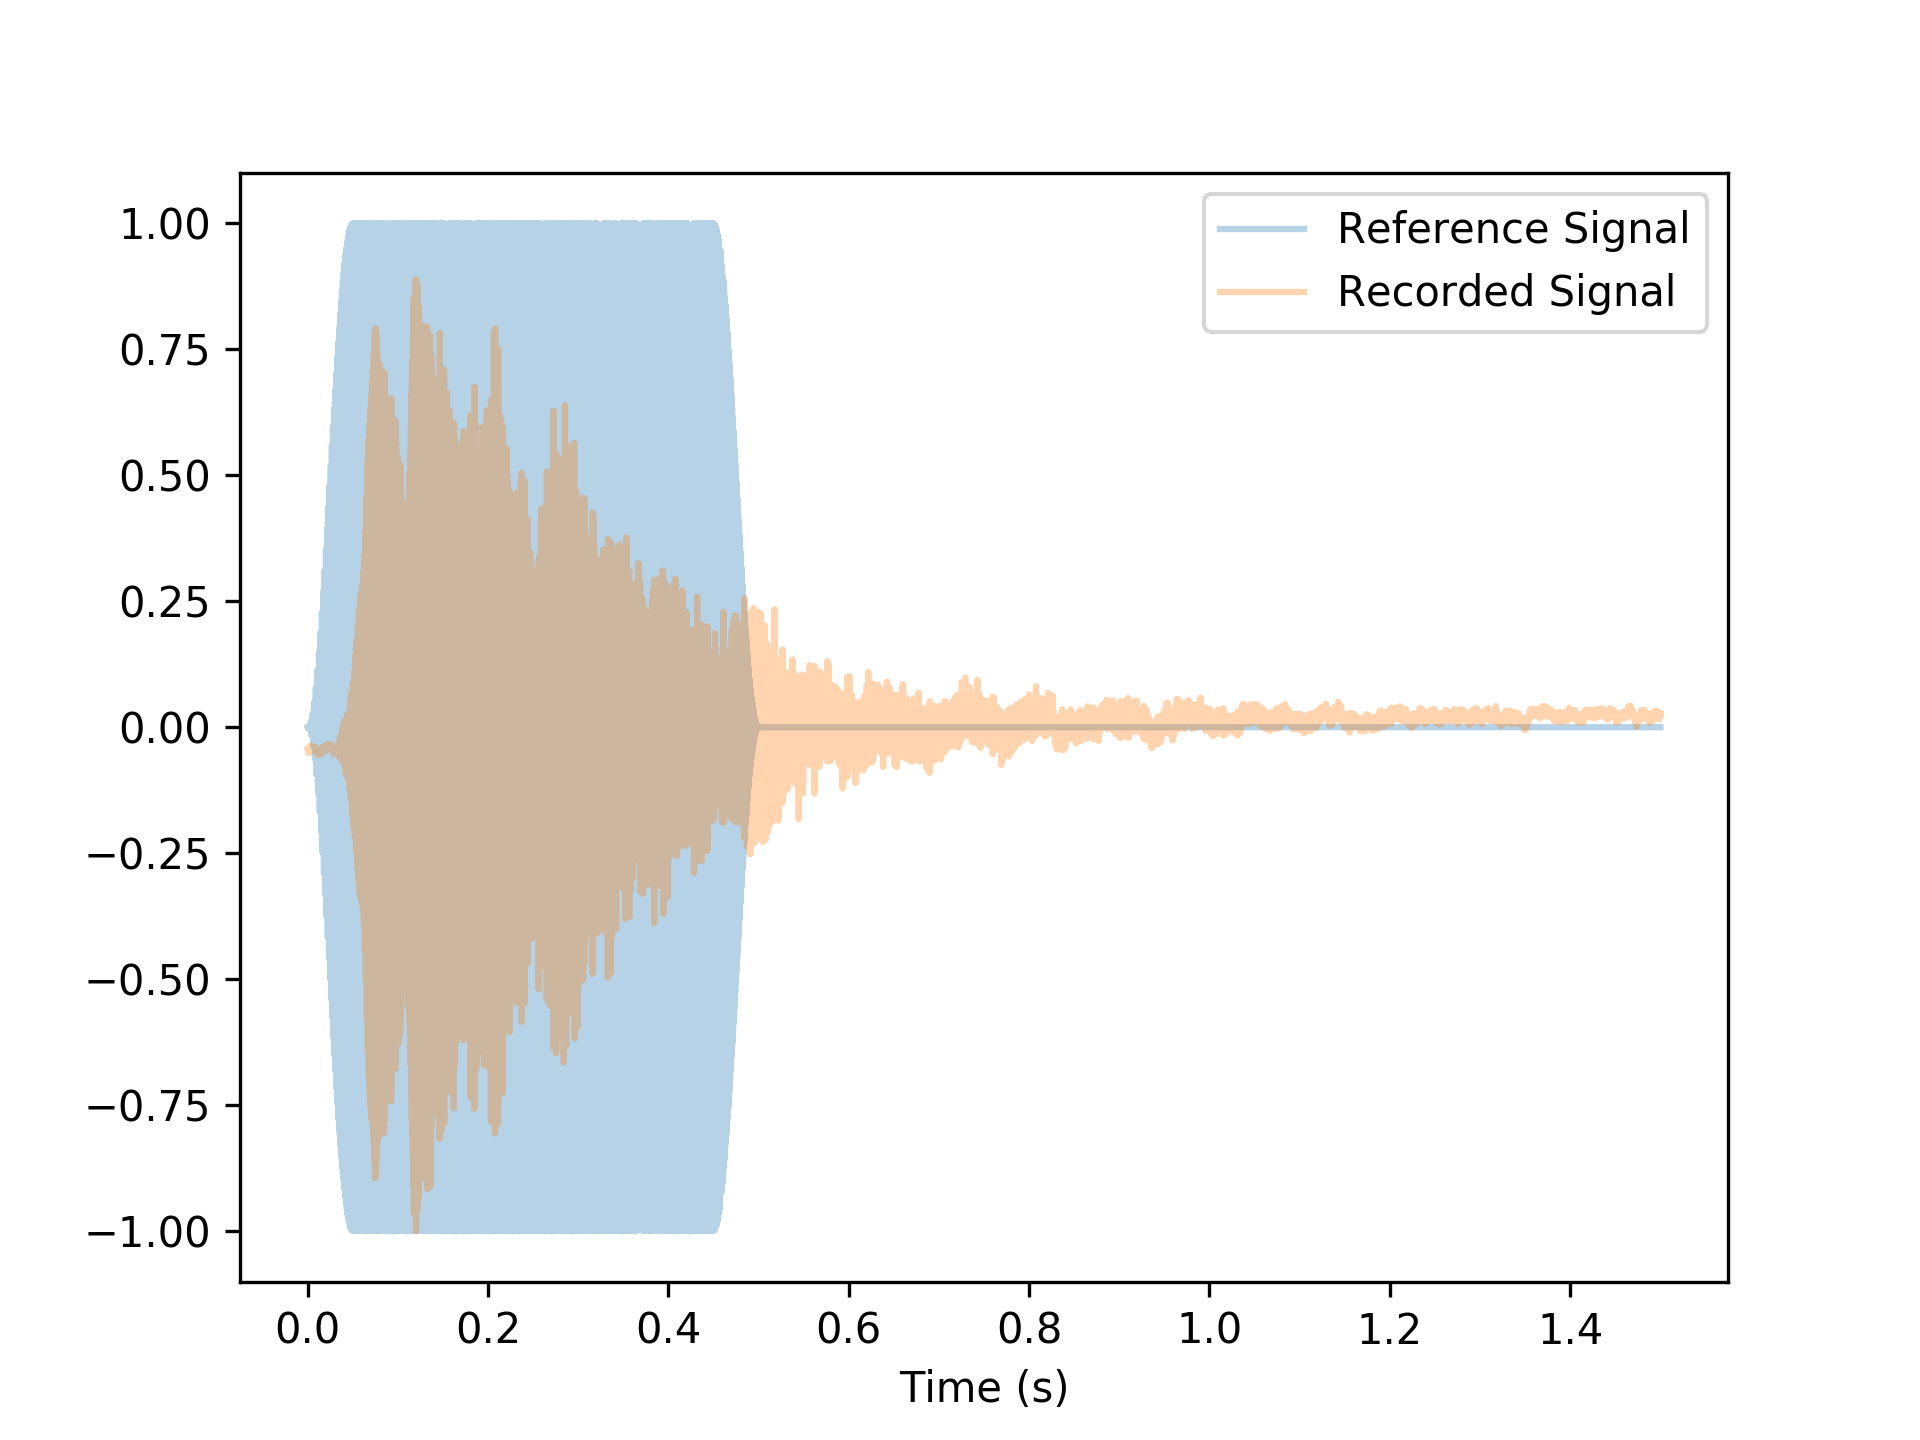
\includegraphics[width=0.5\textwidth]{images/signal_example.png} }}
	\subfloat{{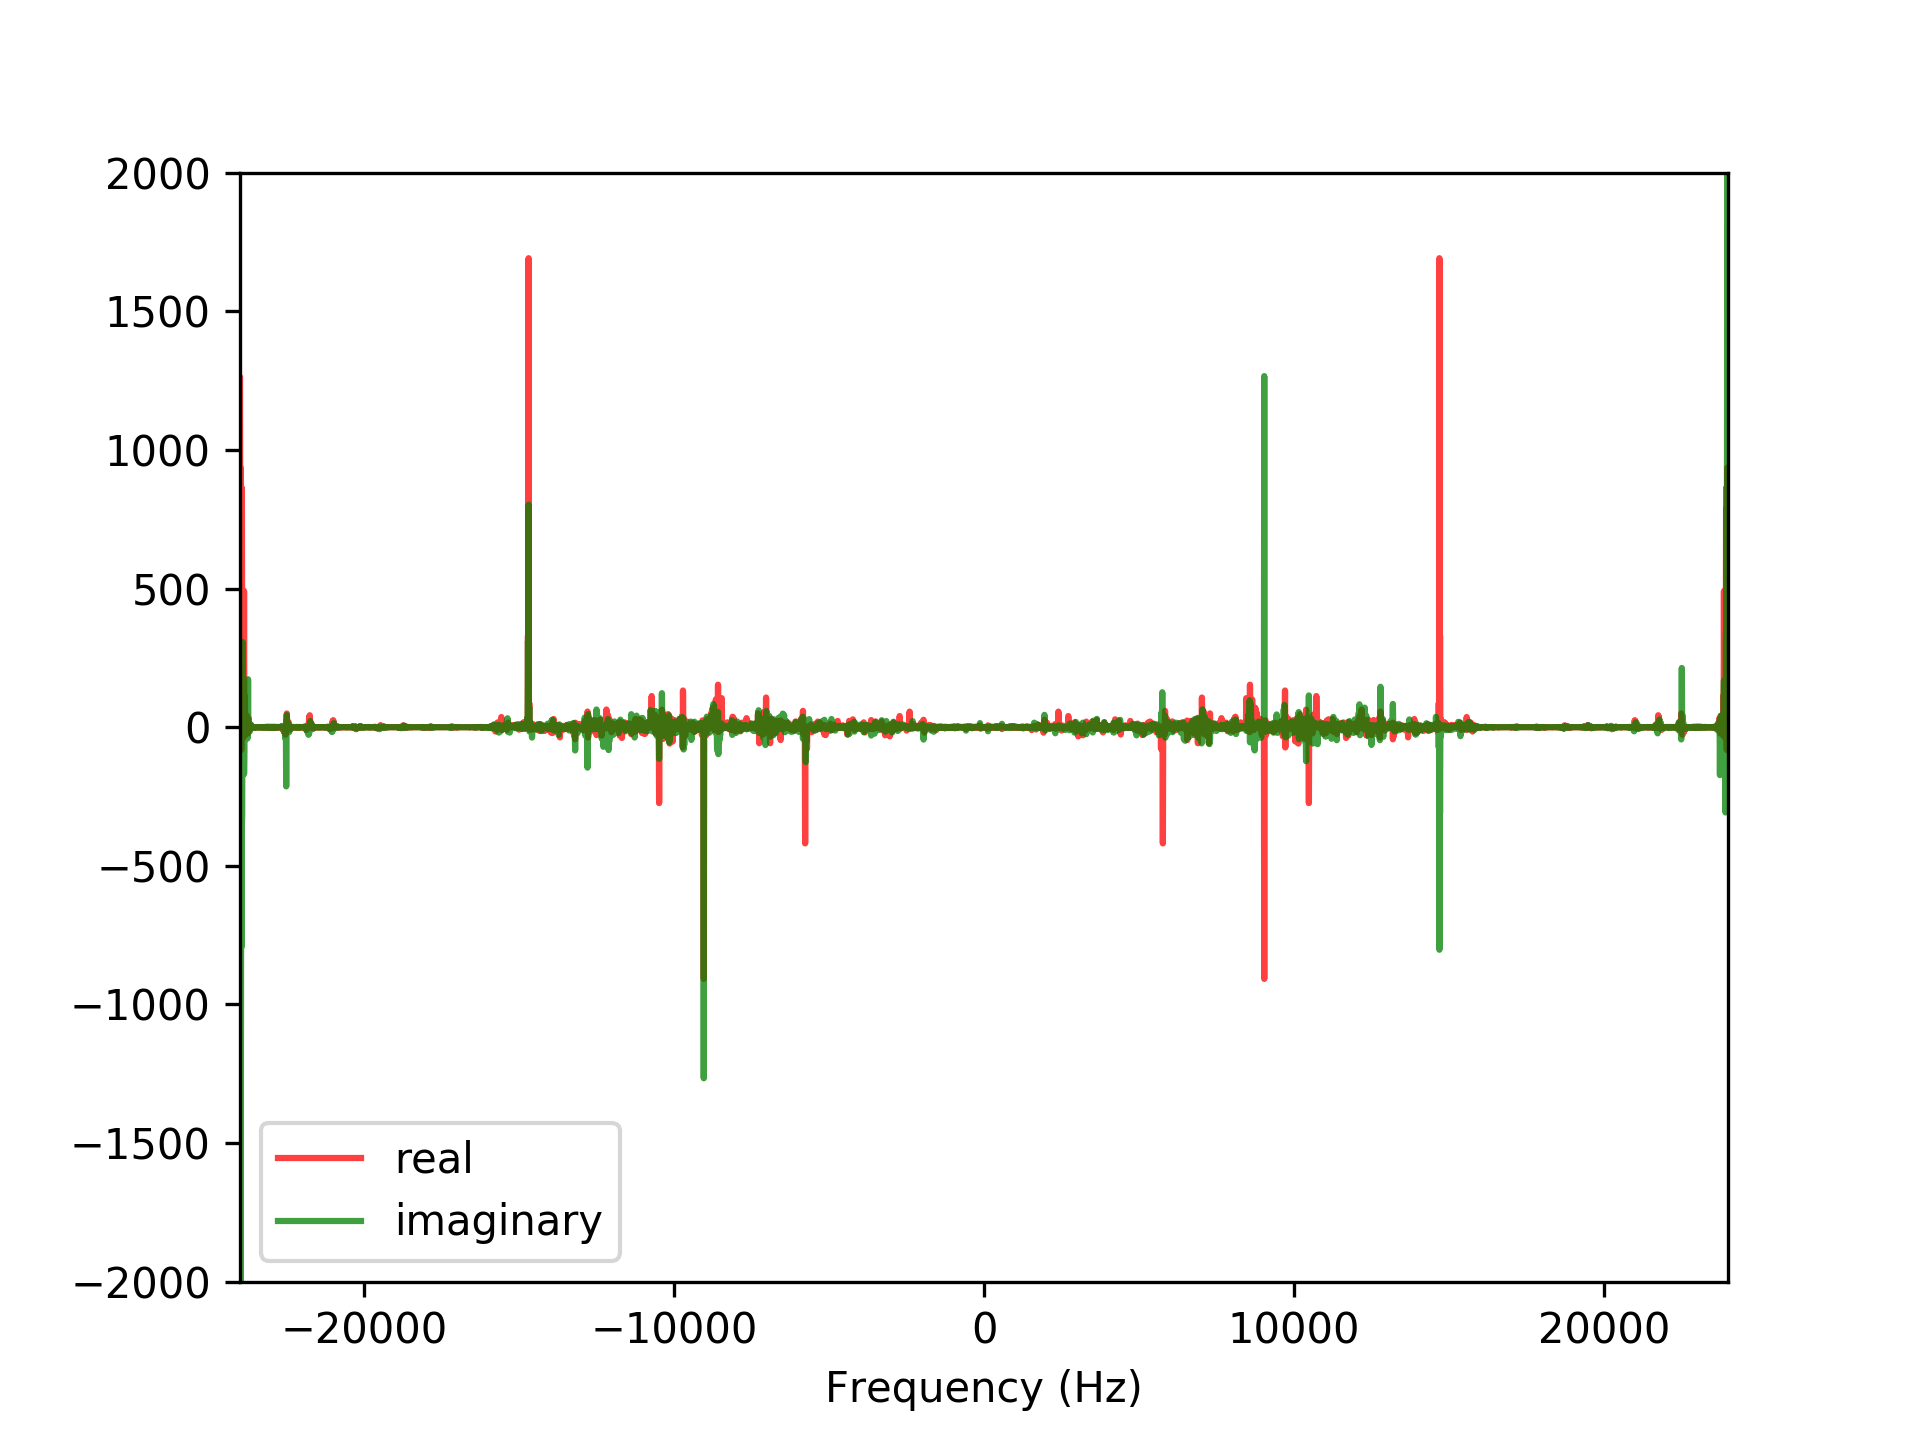
\includegraphics[width=0.5\textwidth]{images/response_example.png} }}
	\caption{
		On the left in blue, the chirp signal with a frequency starting at 200 Hz and going up to 4000 Hz linearly. The chirp signal is 0.5 seconds long and was multiplied with a Tukey window to prevent clicking sounds. In orange the recorded signal and on the right the RIR.
	}
	\label{fig:signal_response_example}
\end{figure}

But it seems that the phase isn't necessary for this use case. When looking at the peaks of the magnitude, RIR at the same position will look similar as illustrated in figure \ref{fig:response-same-room-same-pos}. But that's expectable when looking at the work of Dokmanic \cite{dokmanic_roomrecslam_2016}. Also expectable is that the peaks in magnitude are at a different position when changing the room which can be seen in figure \ref{fig:response-different-room}. More interesting is the RIR of the same room but different positions. It turns out that the RIR is recognizably different in the same room but in different positions which can be seen in figure \ref{fig:response-same-room-different-pos}. Also interesting, peaks in the same room but different positions seem to be at similar positions when moving around (like in figure \ref{fig:dokmanic_roomrecslam}). But when changing the room the peak characteristic will change. That probably leads to a continuous function which is usable for SLAM purposes.

\begin{figure}[h!]
	\centering
	\captionsetup{justification=centering,margin=1cm}
	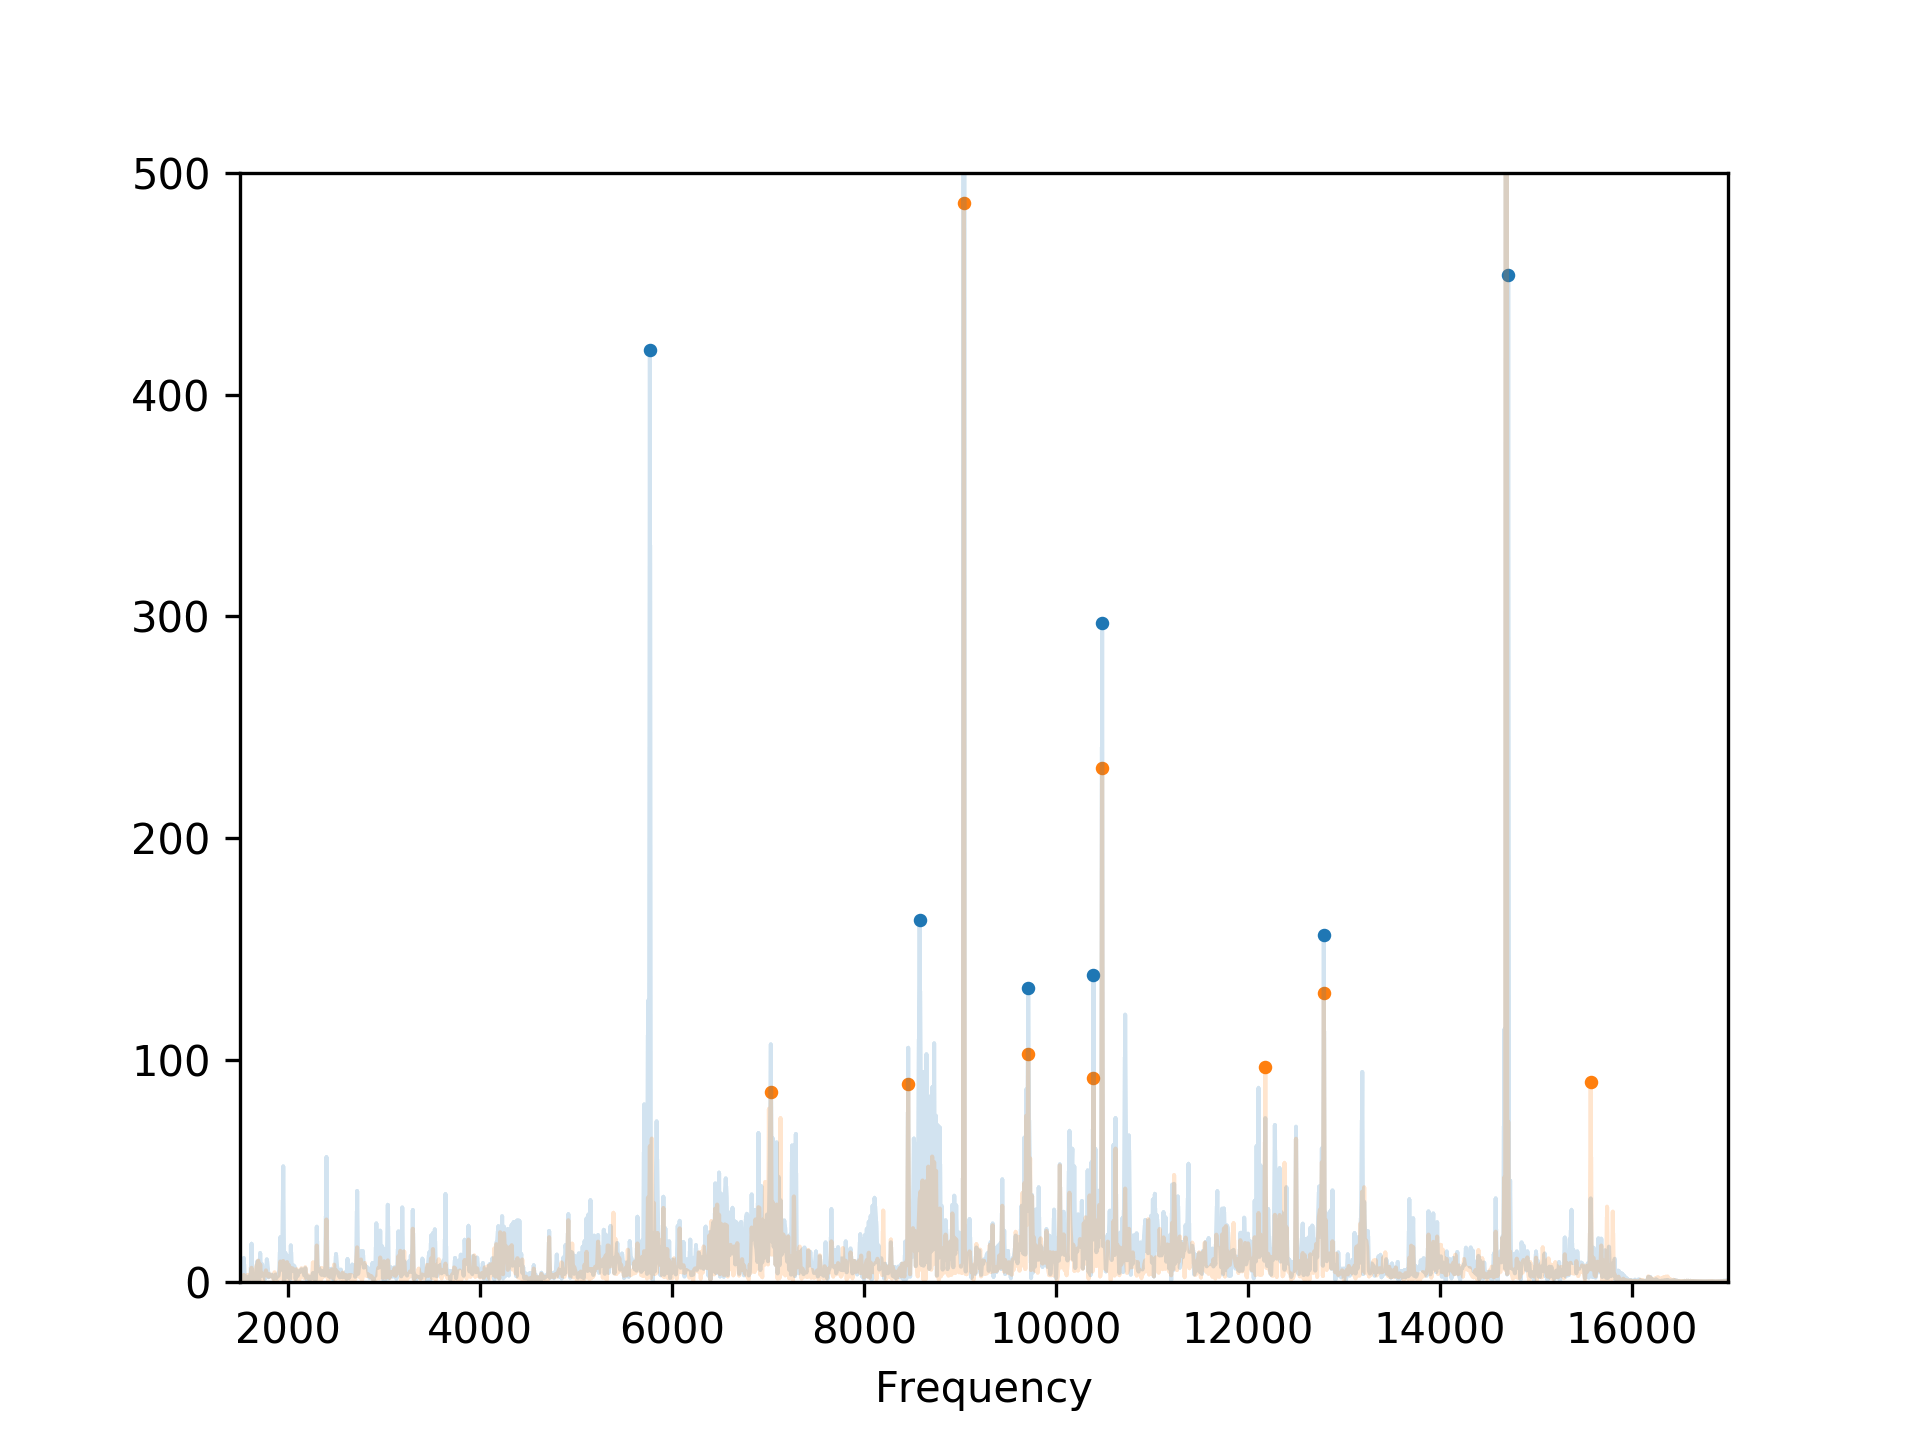
\includegraphics[width=0.49\textwidth]{images/response-same-room-same-pos.png}
	\caption{
		Two RIR of the position but different times. Notice, most of the peaks are at the same position.
	}
	\label{fig:response-same-room-same-pos}
\end{figure}

\begin{figure}[h!]
	\centering
	\captionsetup{justification=centering,margin=1cm}
	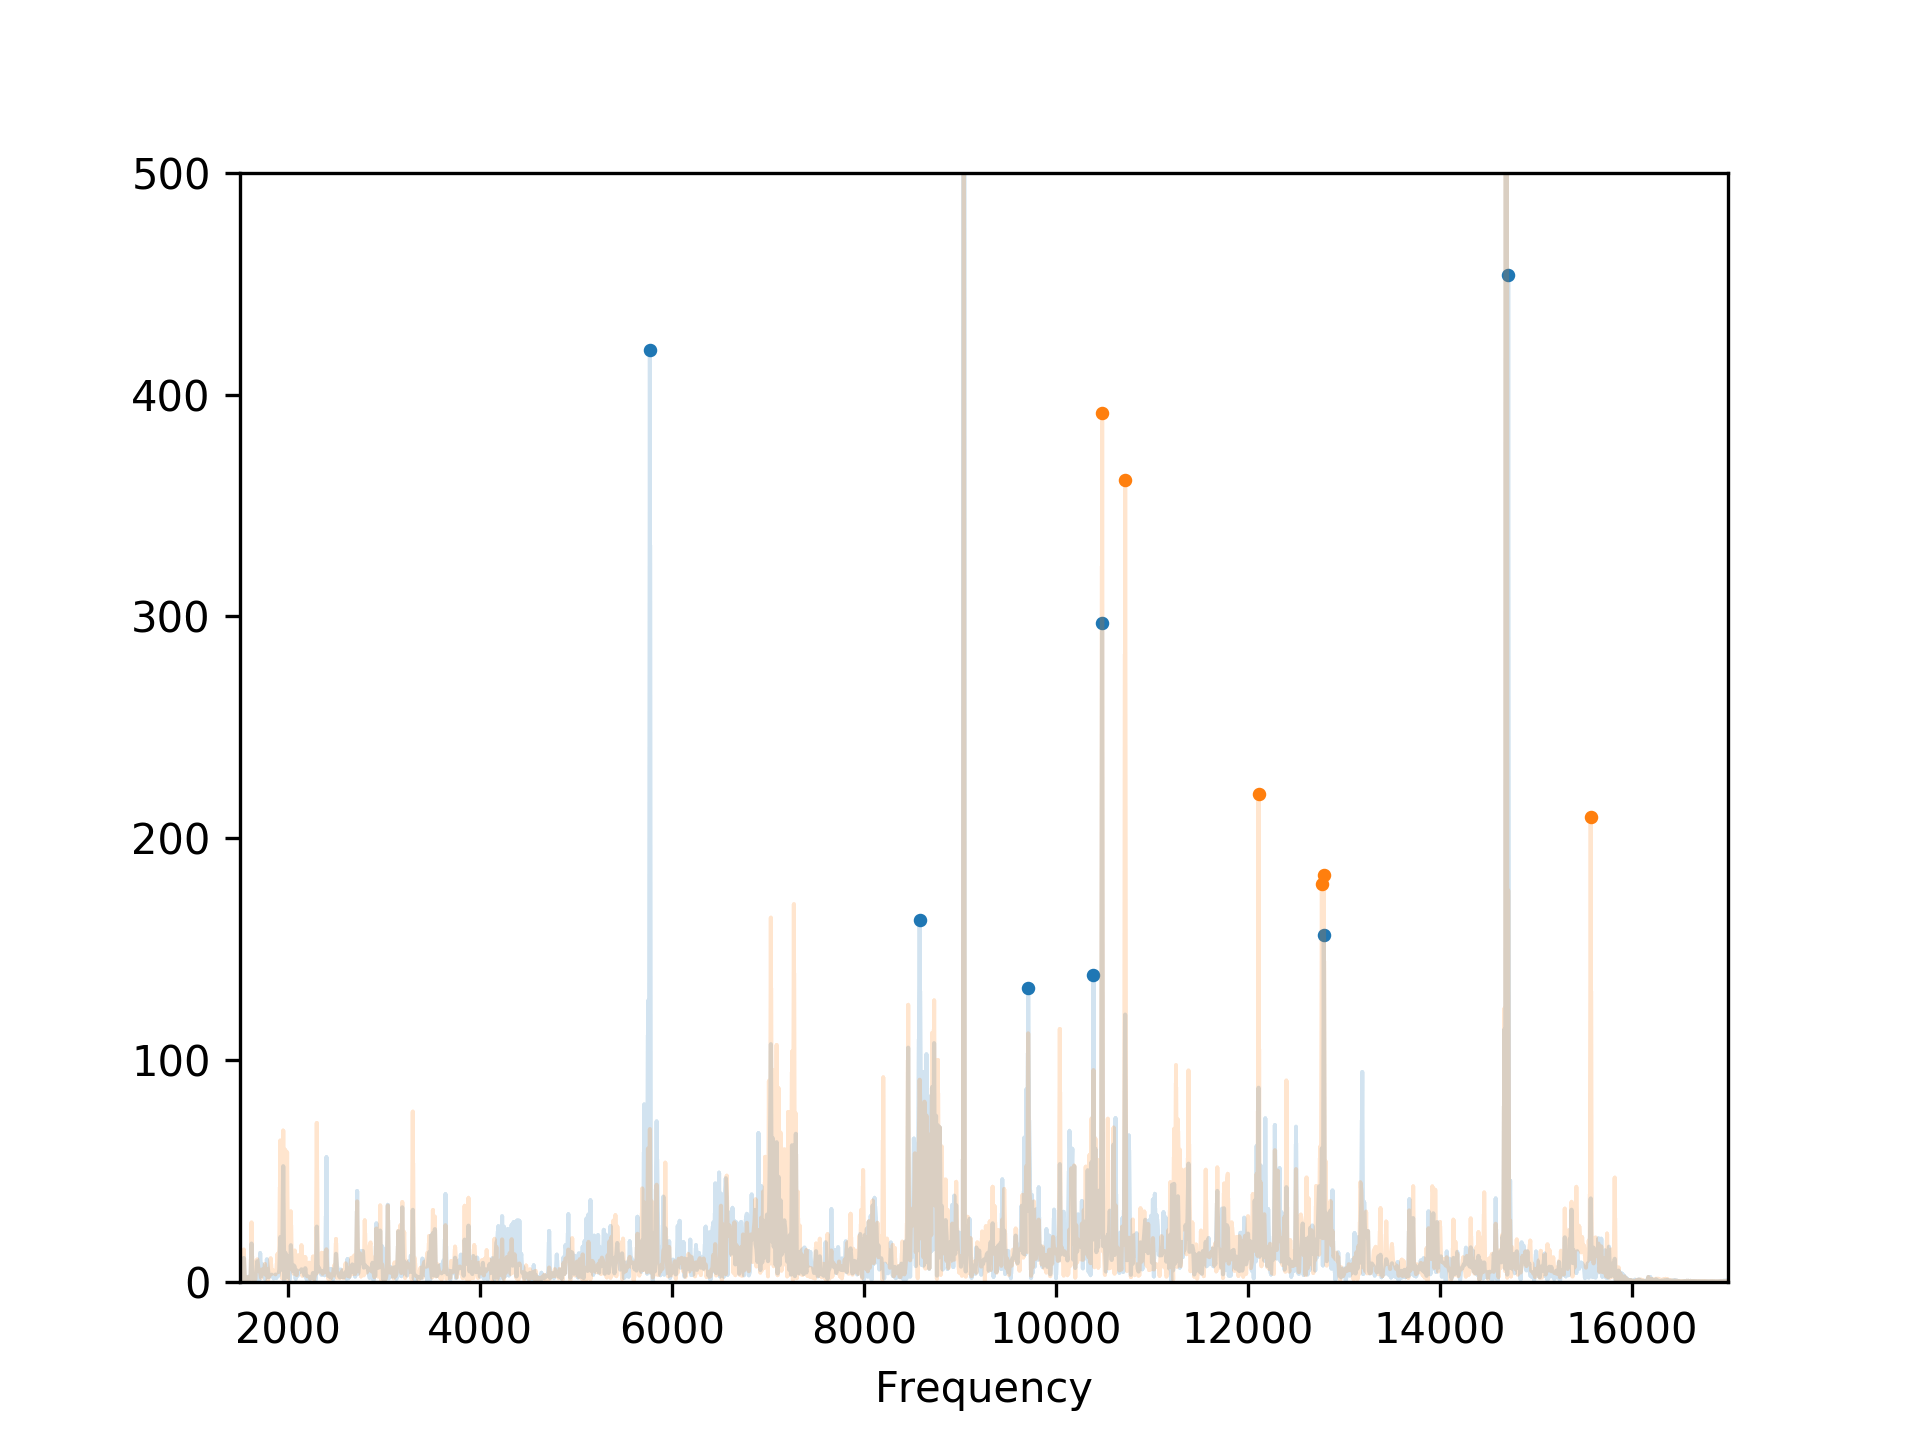
\includegraphics[width=0.49\textwidth]{images/response-different-room.png}
	\caption{
		Two RIR of different rooms. Notice, the peak characteristic has changed.
	}
	\label{fig:response-different-room}
\end{figure}

\begin{figure}[h!]
\centering
\captionsetup{justification=centering,margin=1cm}
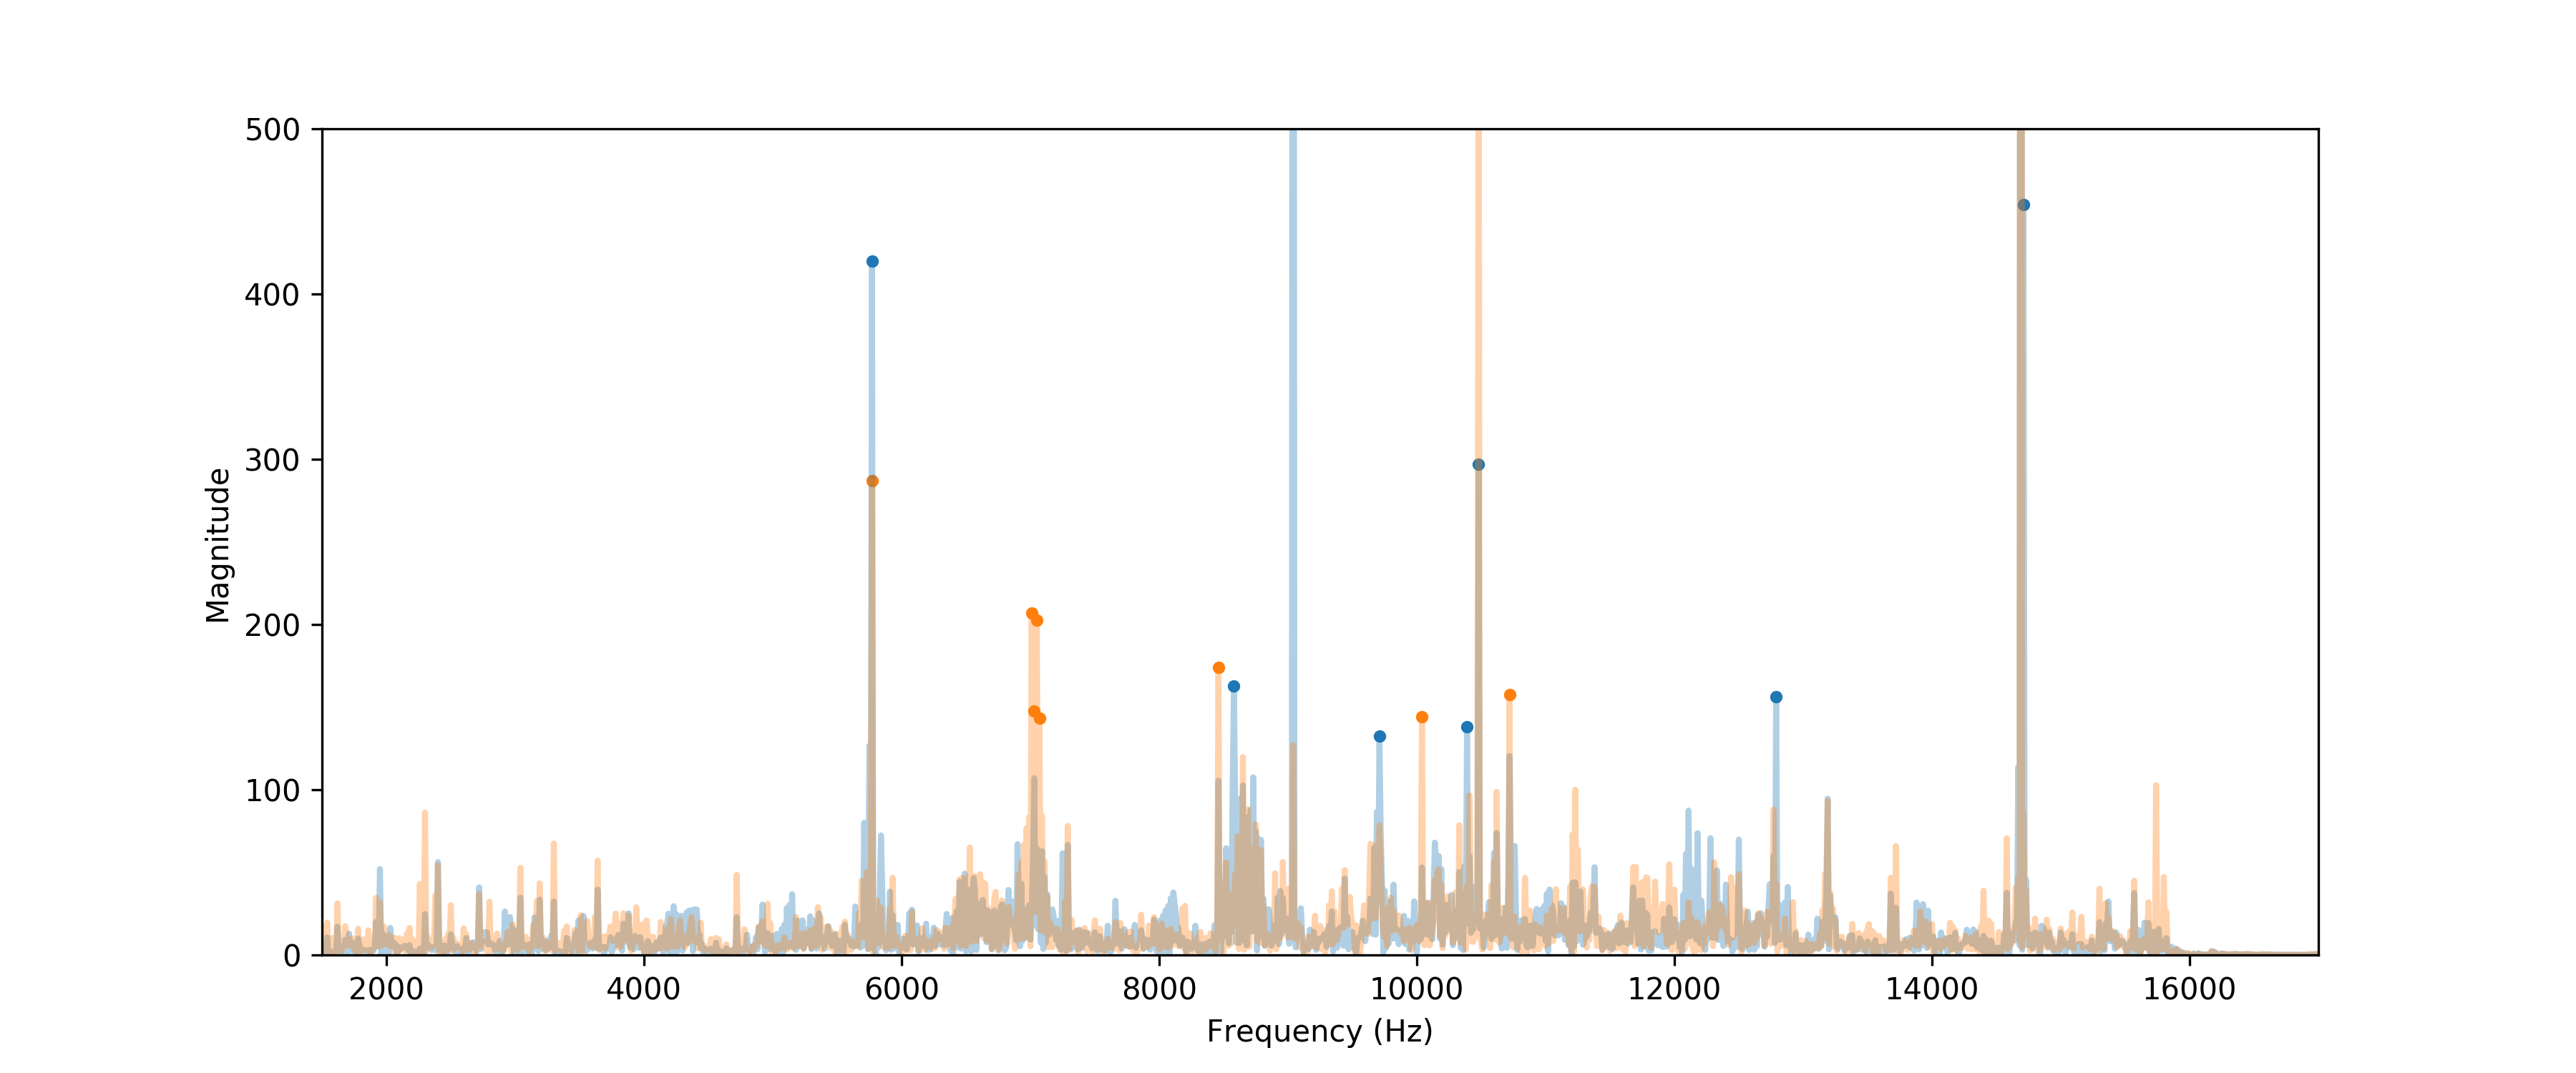
\includegraphics[width=0.49\textwidth]{images/response-same-room-different-pos.png}
\caption{
	Two RIR of the same room but different positions. Notice, the change in peaks is recognizable but some peaks are only shifted slightly.
}
\label{fig:response-same-room-different-pos}
\end{figure}

\section{Project Aims}

The overall project goal is to implement a SLAM approach based on the RIR with a mobile platform equipped with an IMU, speaker, and microphone. To reach that, intermediate targets have to be defined. At first, the aim is to show that the RIR is a continuous function also for moving speakers not only for stationary ones which is already shown by Dokmanic \cite{dokmanic_roomrecslam_2016} as described in Section \ref{sec:acoustic_slam}. For that, data of a moving agent has to be recorded which also can be a human holding the equipment and moving around for first tests. 

Section \ref{sec:acoustic_slam} is showing that the RIR is a continuous function in case of a static speaker. This project wants to show that this is also the case for a speaker and microphone mounted on the same object. After that, based on the RIR a continuous function suitable for real-time SLAM has to be found. Therefore several approaches should be compared. For example, using only the most significant peaks. The RIR itself couldn't be used because of performance issues. When a function suitable for SLAM is found, this function needs to be approximated with a Gaussian process (GP) for SLAM usage. Suitable kernel functions for GP should be compared and the best fitting parameter set up for the kernel should be found. In the end, the SLAM approach needs to be implemented and compared to other SLAM approaches which are based on continuous functions.

When a function suitable for real-time SLAM is found, the SLAM approach has to be implemented, tested, and validated. For implementation, other approaches for continuous SLAM described in Chapter \ref{chap:stat_of_the_art} can be used for orientation. For testing purposes, the performance of the implemented SLAM approach should be examined. Where the performance could be the error or real-time requirements. When it comes to evaluation, the approach could be compared to other approaches that are described in Chapter \ref{chap:stat_of_the_art}. Especially to the one from Dokmanic \cite{dokmanic_roomrecslam_2016} where the project is largely based on.
\section{Work plan}

To reach the goals of this project, the project is divided into six phases. Each phase leads to a milestone at the end of the phase and has also a time buffer of one week. An overview of the work plan can be seen as a Gantt chart in figure \ref{fig:workplan}. Each phase is now explained in detail in the following sections.

\subsection{Data Acquisition}
For the first phase, a workload of six weeks is scheduled. It is also divided into three subphases. Firstly, a phase to understand and analyze the equipment for data recording. In the pre-studies, the microphone and speaker were already used but for the SLAM approach we need sound recordings in combination with position data. For that, several options are given by the Institut which have to be compared and understood. For example the HTC Vive for measuring position data in combination with the robot platform.

During this phase, the next phase can start where data is acquired for later analysis. This data could also have position data but that's not necessary. This data is used to compare different approaches for continuous functions based on the RIR. It also should show later if the RIR with moving speaker will behave similarly to the approach from Dokmanic \cite{dokmanic_roomrecslam_2016} as described in section \ref{sec:acoustic_slam}.

After the analysis data is collected and all equipment is understood, the test and validation data can be gathered. This data should be used later to test and validate the implemented SLAM approach. So it should be a combination of sent output, recorded input, and position data for every timestep t.

The milestone of this phase will be to gather analysis, test, and validation data. If this phase will unexpectedly take much longer so the whole project will be in danger, at least the RIR approach explained in chapter \ref{chap:pre_studies} can be applied to the data to show if the RIR for moving speakers behave continuously. 

\subsection{Data Analysis}
\label{phase:data_analysis}
After the data acquisition phase, the data has to be analyzed in this phase to derive a continuous function suitable for SLAM and approximable with Gaussian Processes in real-time. For this, a workload of seven weeks is scheduled. This phase is also divided into two phases. The first one to analyze the data to find suitable continuous functions and the second phase to compare several approaches for continuous functions.

The milestone in this phase will be to find out the most promising continuous functions derived from the acoustic signal usable for SLAM approaches. If the project needed too much time until this phase, several approaches for continuous functions suitable for SLAM could be published which shows that acoustic SLAM is probably suitable for completely unprepared environments.

\subsection{Gaussian Process Optimization}
This phase will be a short phase with a workload of one week. In this phase, the Gaussian processes will be optimized for the different continuous functions given by the phase before. So the milestone will be a set of optimal Gaussian processes for the given functions. If no time after this phase is left for further work, a paper of the functions suitable for SLAM with some plots of the continuous function in space could be published.

\subsection{Implementing Test Environment and SLAM Approach}
A workload of five weeks is scheduled for this phase. This phase is also divided into three phases where one phase is implementing a test environment to simulate a virtual robot with the data given by the phase described in \ref{phase:data_analysis}. This test environment is also used for later validation purposes. The next phase is to plot a map of the continuous functions to finally see if it's suitable for SLAM and if there are any errors or other issues within the data or with the derived functions. In the end, a SLAM approach will be implemented which is also the milestone of this phase. As in the phase before, if no time is left the derived functions and plots showing the continuous functions suitable for SLAM can be published. 

\subsection{Test and Validation}
The test and validation phase is scheduled with a workload of three weeks and is divided into three subphases. First testing the SLAM approach given by the phase before in the test environment. After that, the SLAM approach should be tested on real data with a robot platform. At the end, the results should be compared to other approaches especially to the one from Dokmanic \cite{dokmanic_roomrecslam_2016} described in section \ref{sec:acoustic_slam}. The milestone of this phase will be the validation of this approach and the comparison to others. If the time is getting short, the test on real data could be canceled and the SLAM approach will only be tested in the virtual environment on the data given by the first phase described in \ref{phase:data_analysis}. 

\subsection{Paper Writing}
In the end, all knowledge of the project has to be gathered and written down into a paper. For that, a workload of three weeks is scheduled. It seems a little bit short but every phase should produce a short document with the milestone. Also, each phase has a buffer of one week. So if every phase before will work as planned, there will be six weeks buffer left for this phase. The milestone of this phase will be the paper. 

\begin{figure}[hp]
	\centering
	\captionsetup{justification=centering,margin=1cm}
	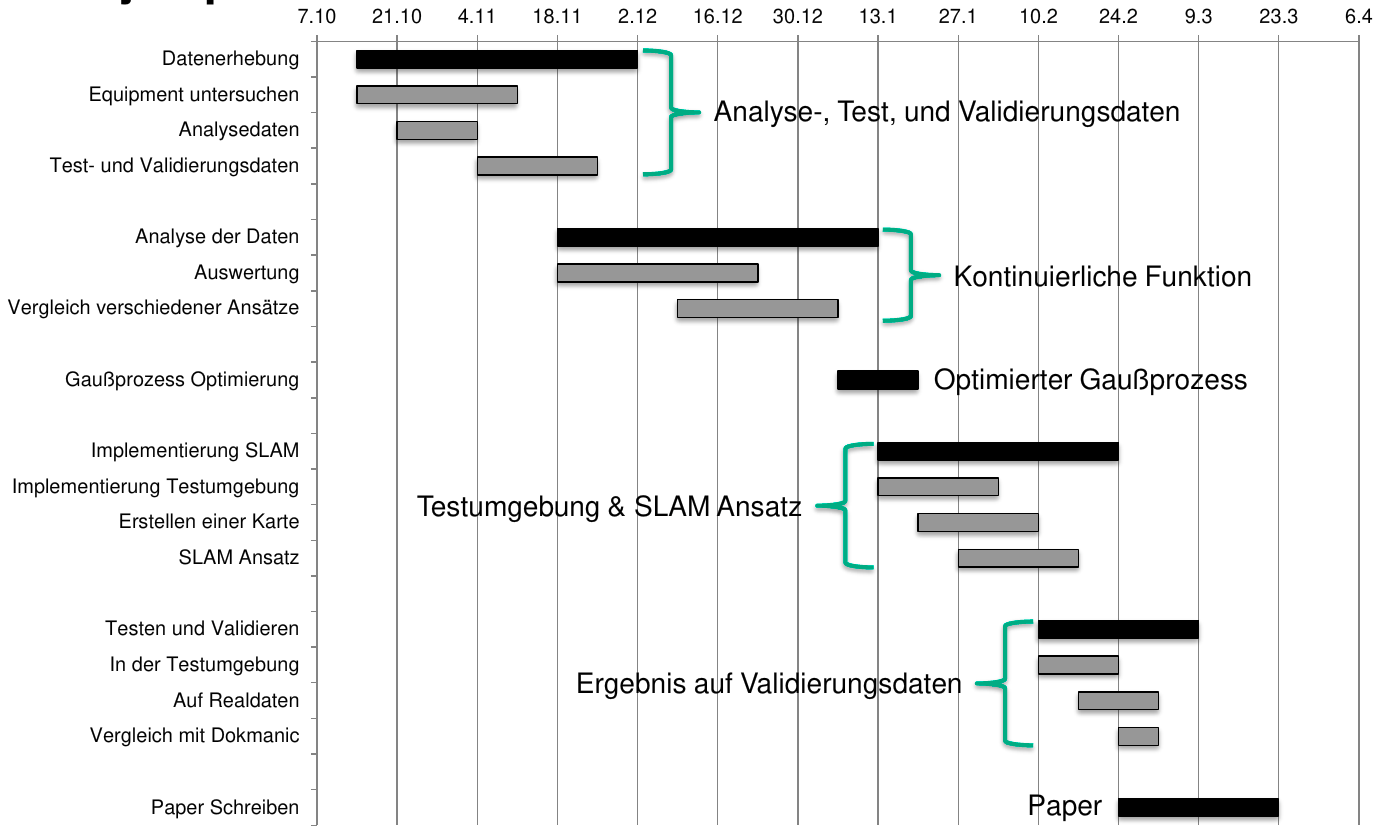
\includegraphics[width=\textwidth]{images/workplan.png}
	\caption{
		This is the Gantt chart to illustrate the project plan. TODO CHANGE TO ENGLISH
	}
	\label{fig:workplan}
\end{figure}

\nocite{*}


\bibliography{sources}{}

\bibliographystyle{ieeetr}



\end{document}
